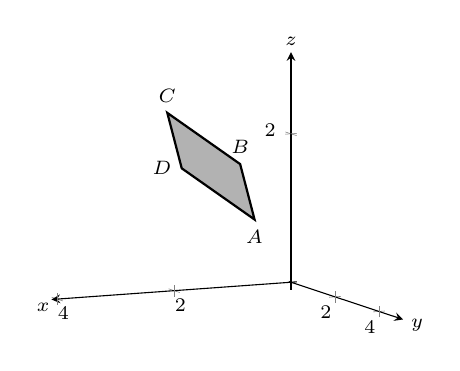
\begin{tikzpicture}
\begin{axis}%
[width=175pt,tick label style={font=\scriptsize},axis on top,
			axis lines=center,
			view={155}{10},
			name=myplot,
			%xtick=\empty,
			%ytick=\empty,
			%ztick=\empty,
			ymin=-.1,ymax=5.1,
			xmin=-.1,xmax=4.1,
			zmin=-.1, zmax=3.1,
			every axis x label/.style={at={(axis cs:\pgfkeysvalueof{/pgfplots/xmax},0,0)},xshift=-3pt,yshift=-3pt},
				xlabel={\scriptsize $x$},
			every axis y label/.style={at={(axis cs:0,\pgfkeysvalueof{/pgfplots/ymax},0)},xshift=5pt,yshift=-2pt},
				ylabel={\scriptsize $y$},
				every axis z label/.style={at={(axis cs:0,0,\pgfkeysvalueof{/pgfplots/zmax})},xshift=0pt,yshift=4pt},
				zlabel={\scriptsize $z$}
			]


\filldraw [draw=black,fill=black!30,thick] (axis cs: 1,1,1) node [below] {\scriptsize $A$} -- (axis cs:2,3,2) node [above] {\scriptsize $B$} -- (axis cs: 4,5,3)node [above] {\scriptsize $C$} -- (axis cs: 3,3,2) node [left] {\scriptsize $D$}-- cycle;

%\threedlines{4}{5}{3}
%\threedlines{2}{3}{2}

%\addplot3[domain=-.1:1,y domain=-.1:1,surf,faceted color=black!20,samples=10,black!10] {-.1*x+y+1};
%
%\draw[>=stealth,->,thick] (axis cs:.1,.1,1.09) -- (axis cs: .7,.1,1.03) node [ left] {\scriptsize $\vec u$};
%
%\filldraw[black] (axis cs: .1,.1,1.09) circle (1pt);
%
%\draw[>=stealth,->,thick] (axis cs:.1,.1,1.09) -- (axis cs: .1,.8,1.79) node [right] {\scriptsize $\vec v$};
%
%\addplot3[domain=0:90,samples y=0,black,thick] ({.3*cos(x)+.1},{.3*sin(x)+.1},{-.1*(.3*cos(x)+.1)+(.3*sin(x)+.1)+1});
%
%\draw (axis cs: .5,.4,1.36) node  {\scriptsize $\theta$};

%\draw (axis cs: 0,0,\pgfkeysvalueof{/pgfplots/zmax}) node [shift={(0,0,20pt)}]{\scriptsize $z$};

%\draw (axis cs: 0,\pgfkeysvalueof{/pgfplots/ymax},0) node [shift={(0,2pt,0)}]{\scriptsize $y$};

%\draw (axis cs: \pgfkeysvalueof{/pgfplots/xmax},0,0) node [shift={(6pt,0,0)}]{\scriptsize $x$};

\end{axis}
%\node [right] at (myplot.right of origin)[shift={(-20pt,-8pt)}] {\scriptsize $y$};
%\node [above] at (myplot.above origin) [shift={(0,-5pt)}] {\scriptsize $z$};
\end{tikzpicture}









